%%%%%%%%%%%%%%%%%%%%%%%%
%% START HEADER MATERIAL
\documentclass[letterpaper]{article} % use larger type; default would be 10pt
\usepackage[utf8]{inputenc}

%%% PAGE DIMENSIONS
\usepackage[margin=1in]{geometry} % to change the page dimensions
\geometry{letterpaper}

%%% PACKAGES
\usepackage{booktabs} % for much better looking tables
\usepackage[format=hang,font=small,labelfont=bf, labelsep=period,
margin=40pt]{caption}
\usepackage{subfig} % make it possible to include more than one captioned figure/table in a single float
\usepackage{float}
\usepackage{graphicx}    % So we can include graphics easily
\usepackage{hyperref} %unusual: for hyperlinking and other effects
\usepackage{comment}
\markright{Grinders.Rnw}   % EDIT THIS TO USE THE ACTUAL RNW FILE NAME!

%%% HEADERS & FOOTERS
\usepackage{fancyhdr} % This should be set AFTER setting up the page geometry
\pagestyle{fancy} % options: empty , plain , fancy
\renewcommand{\headrulewidth}{0pt} % customize the layout...
\lhead{}\chead{}\rhead{}
\lfoot{}\cfoot{\thepage}\rfoot{}

\newenvironment{list1}{
  \begin{list}{\ding{113}}{%
      \setlength{\itemsep}{0in}
      \setlength{\parsep}{0in} \setlength{\parskip}{0in}
      \setlength{\topsep}{0in} \setlength{\partopsep}{0in} 
      \setlength{\leftmargin}{0.17in}}}{\end{list}}
\newenvironment{list2}{
  \begin{list}{$\bullet$}{%
      \setlength{\itemsep}{0in}
      \setlength{\parsep}{0in} \setlength{\parskip}{0in}
      \setlength{\topsep}{0in} \setlength{\partopsep}{0in} 
      \setlength{\leftmargin}{0.2in}}}{\end{list}}
      
%%% SECTION TITLE APPEARANCE
\usepackage{sectsty}
\allsectionsfont{\sffamily\mdseries\upshape}

\usepackage{dcolumn}

%%% OBVIOUSLY, YOU SHOULD EDIT THESE EACH TIME!
\title{Research Choices Within and Between Disciplines}
\author{Nandana Sengupta and Kyle Bocinsky}


\usepackage{Sweave}
\begin{document} % required to get started
\maketitle
%% END HEADER MATERIAL
%%%%%%%%%%%%%%%%%%%%%%%%
Consider the following situation: \emph{Academics choose research topics}.

\begin{list1}
\item[] Model, using whatever techniques you wish, the above scenario.
\begin{list2}
%\vspace*{.05in}
\item[] Explicitly state your model and key assumptions. %\href{http://village.anth.wsu.edu/~bocinsky/bocinsky_thesis_final.pdf}{[pdf}]
\item[] Summarize key results.
\item[] Suggest some potentially interesting future directions and questions for the model.
\end{list2}
\item[] Suggest some standard social science scenarios that could be usefully modeled using such a process.
\end{list1}

\section*{Introduction}
We are interested in modeling patterns of topic and strategy choice in academic research. Specifically, we are trying to replicate are the booms and busts in popularity of certain research topics and also the rare event of a topic becoming so popular that it takes over a given discipline. We also model research choices based on individual characteristics and try to explain the recent trend in interdisciplinary research as the exploitation of easy short term gains from choosing to do interdisciplinary work. This occurs even if it does not appear to be the obvious choice in terms of research potential within the different disciplines.
\newline  
\newline
We consider the following two models of research choice:
\begin{enumerate}
\item
Research choices within disciplines
\item
Research choices between disciplines
\end{enumerate}
\textbf{Key assumptions and Factors Driving the Model:}
\begin{enumerate}
\item
Our major assumption is regarding the initialization of the model. We assume that each new researcher has an equal likelihood of choosing any one of the existing disciplines. For the second model, we assume that more successful researchers are better able to produce academic `progeny,' and that the supply of graduate students in any given discipline is relatively without limit.
\item
We also assume for simplicity that the total population of researchers stays constant throughout the length of the analysis. 
\item
The driving factors in both models is what we term the ``growth-rate'' of the disciplines. We define this as the proportion of new projects in a given discipline over the entire body of work in that discipline. A high (or low) growth rate therefore is a measure of the relative fertility (or stagnation) of that discipline.  
\end{enumerate}
\textbf{}

%%%%%%%% MODEL 1 %%%%%%%%
\section{Modeling research choice within disciplines}
The simplest model we consider has N academics (researchers) choosing between M research areas. We allow researches to move freely between the areas thus the natural motivation for the model is that of research choices \textit{within} a given discipline. We want to study the evolution of the relative popularity of different research areas. The choice of area is determined by last period's growth rate. We then extend the model by introducing the possibility of a paradigm shift (which is a rare event) which renders the discipline ``young'' again leading to an impetus in the growth rate of the area.  
\newpage
\subsection{Algorithm}
\begin{enumerate}
\item
In each period $t$ the $N$ agents are distributed into $M$ areas according to a multinomial distribution with probability weights $p_t(m)$. In the first period each of the M disciplines is equally likely.
\item Therefore $p_1(m) = 1/M$  $\forall m \in M$. Each agent produces one paper in each time period.  
\item
Each agent calculates the growth rate of area ($m\in M$) at time $t$;$g_t(m)$ as the ratio of number of new papers written in the field in period $t$; ($n_t(m)$) and the the total body of work in the area up till time $t$; $N_t(m)$. Therefore $g_t(m) = \frac{n_t(m)}{N_t(m)}$ where $N_t(m) = N_{t-1}(m) + n_t(m)$. 
\item
The relative weight of growth of an area over the sum of growth rates of all areas determines the probability weights for the distribution of agents for the next period. Therefore $p_{t+1}(m) = \frac{g_t(m)}{\Sigma_{k=1}^{M} g_t(k)}$. 
\item
Steps $1-3$ are repeated for $T$ trials and the evolution of $n_t(m)$, $N_t(m)$ and $g_t(m)$ is studied.
\item
\textbf{With Paradigm Shifts}: In the extension with paradigm shifts we allow for the possibility (extremely rare) of a given paper being a game changer that renders an area "young" again and provides impetus to the growth rate of the area. We model the probability of a given paper of leading to a paradigm shift as $p^{para}=(0.1/N)$. Thus assuming independence across agents, the probability of a paradigm shift in a given area at $t$ is $p_{t}^{para}(m)= \frac{n_t(m).(0.1)}{N}$. This implies $g_t(m)=1$ and the relative probability weight $p_{t+1}(m)$ jumps up.
\end{enumerate}
\newpage
\subsection{Results for Model 1}
Graphical representation of the results:
\begin{figure}[H]
\begin{center}
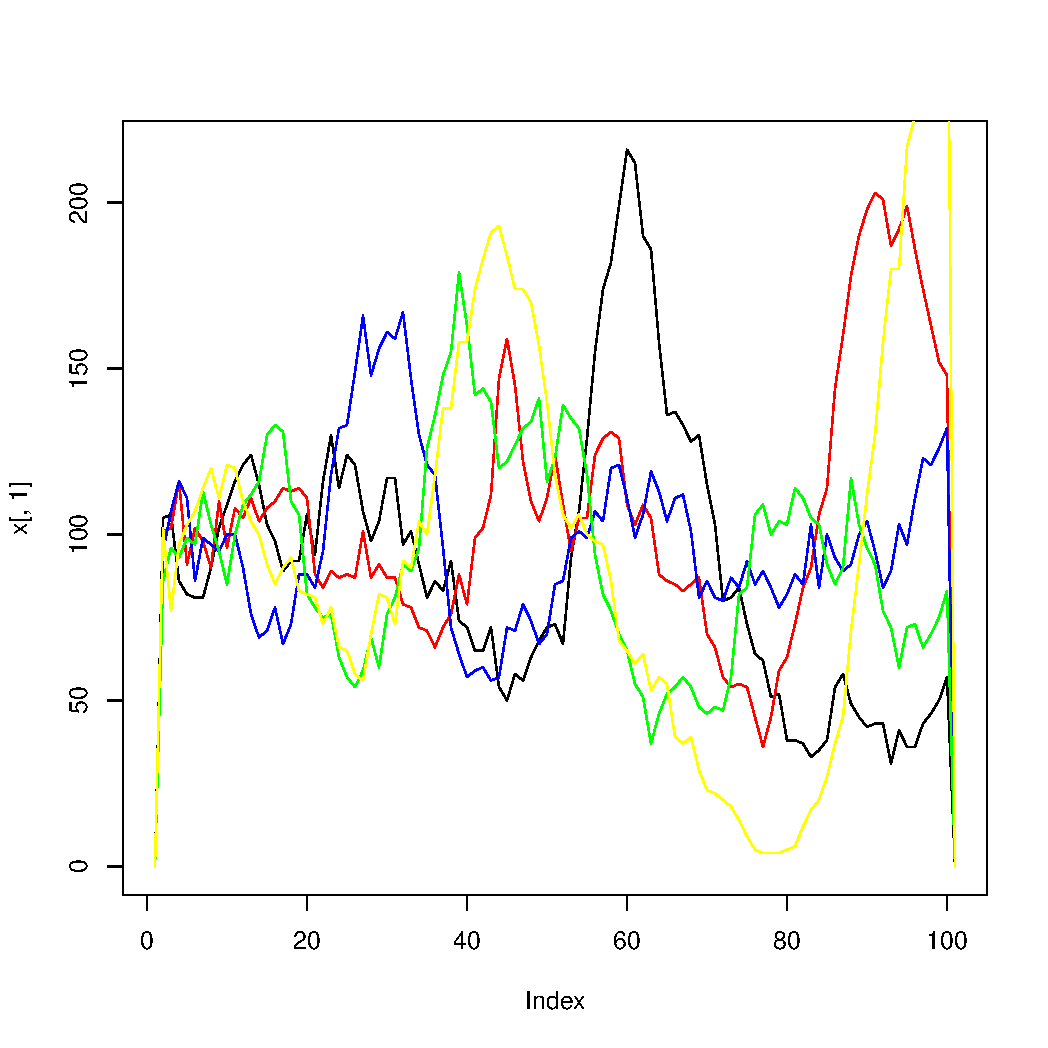
\includegraphics[width=3in]{newres.pdf}
\end{center}
\caption{New Research Per Area}
\end{figure}
\begin{figure}[H]
\begin{center}
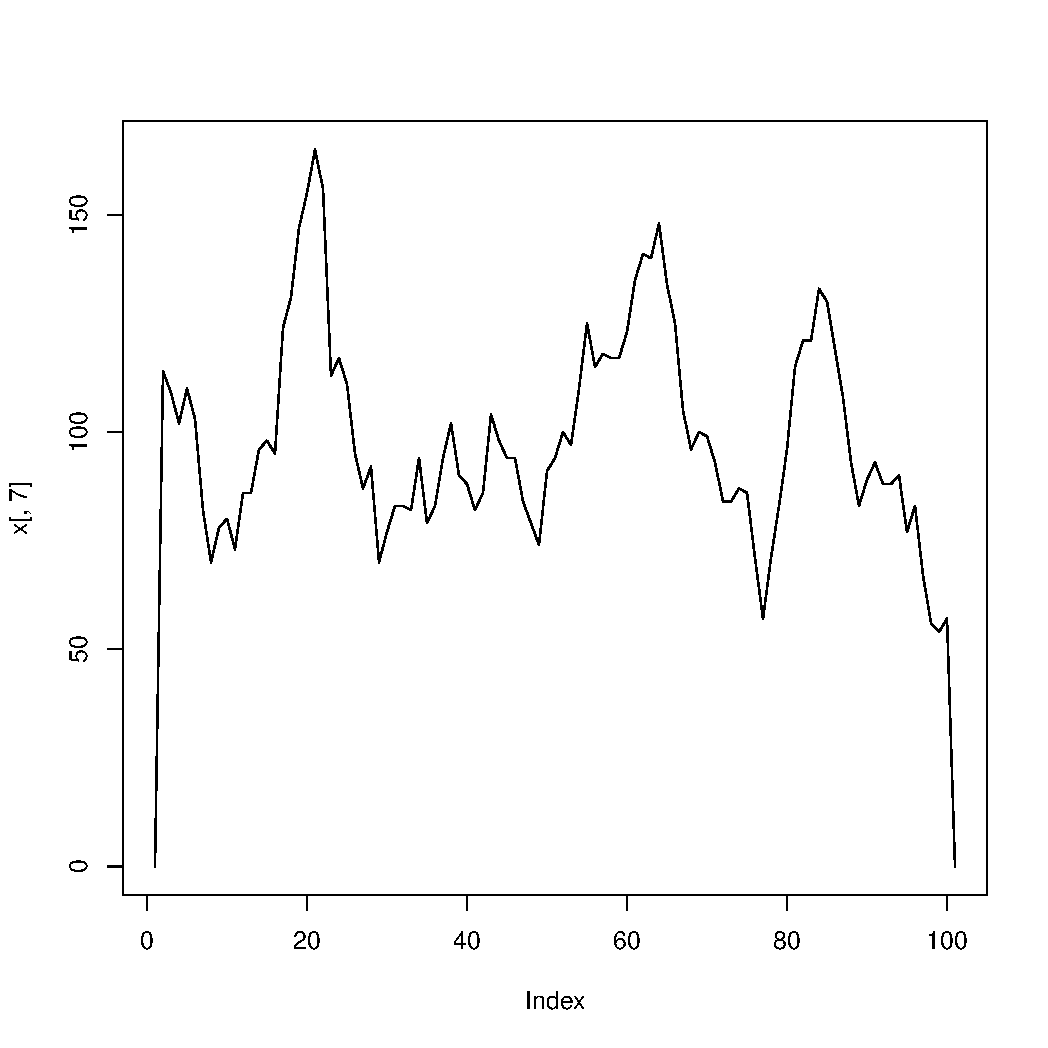
\includegraphics[width=3in]{newres1.pdf}
\end{center}
\caption{New Research in a Given Area : Cycles}
\end{figure}
\begin{figure}[H]
\begin{center}
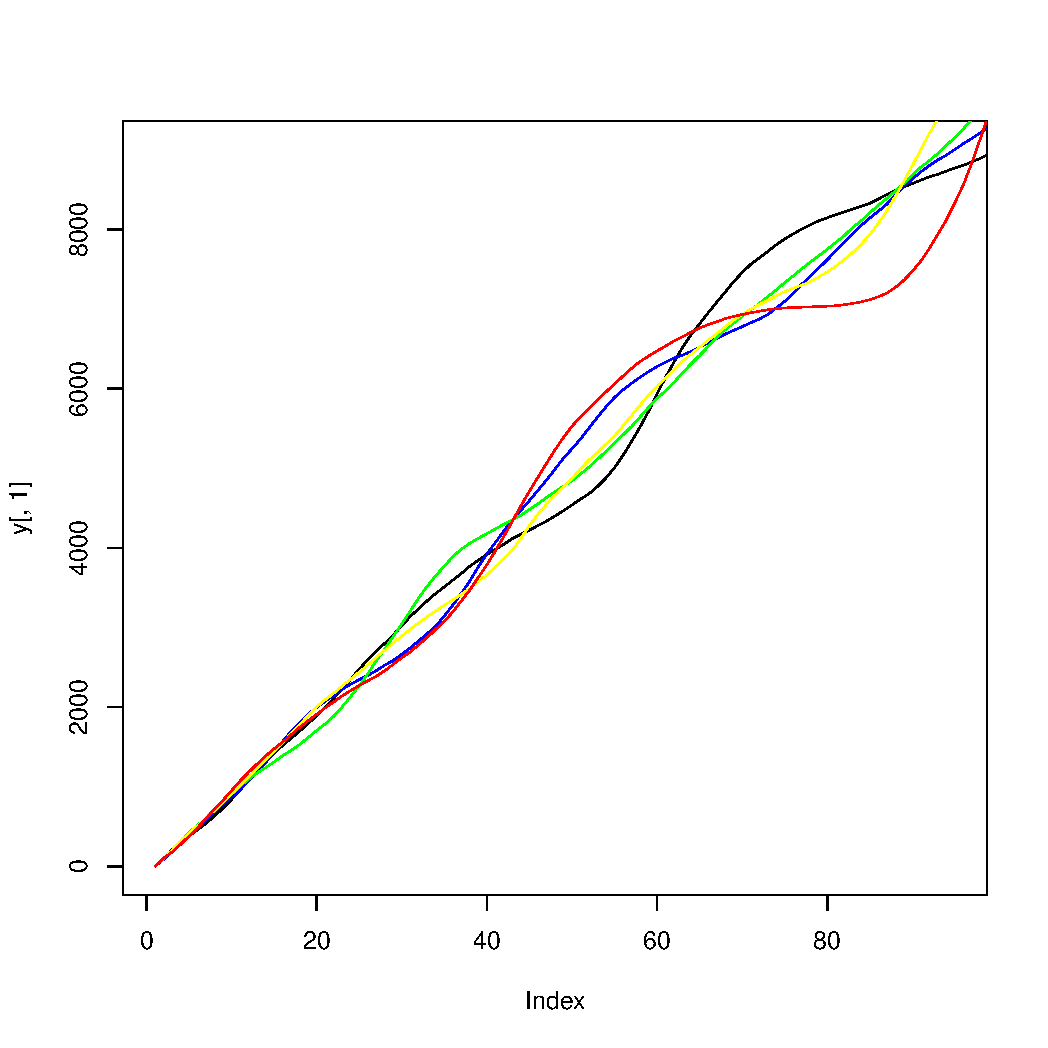
\includegraphics[width=3in]{totalres.pdf}
\end{center}
\caption{Total Research Per Area}
\end{figure}
\begin{figure}[H]
\begin{center}
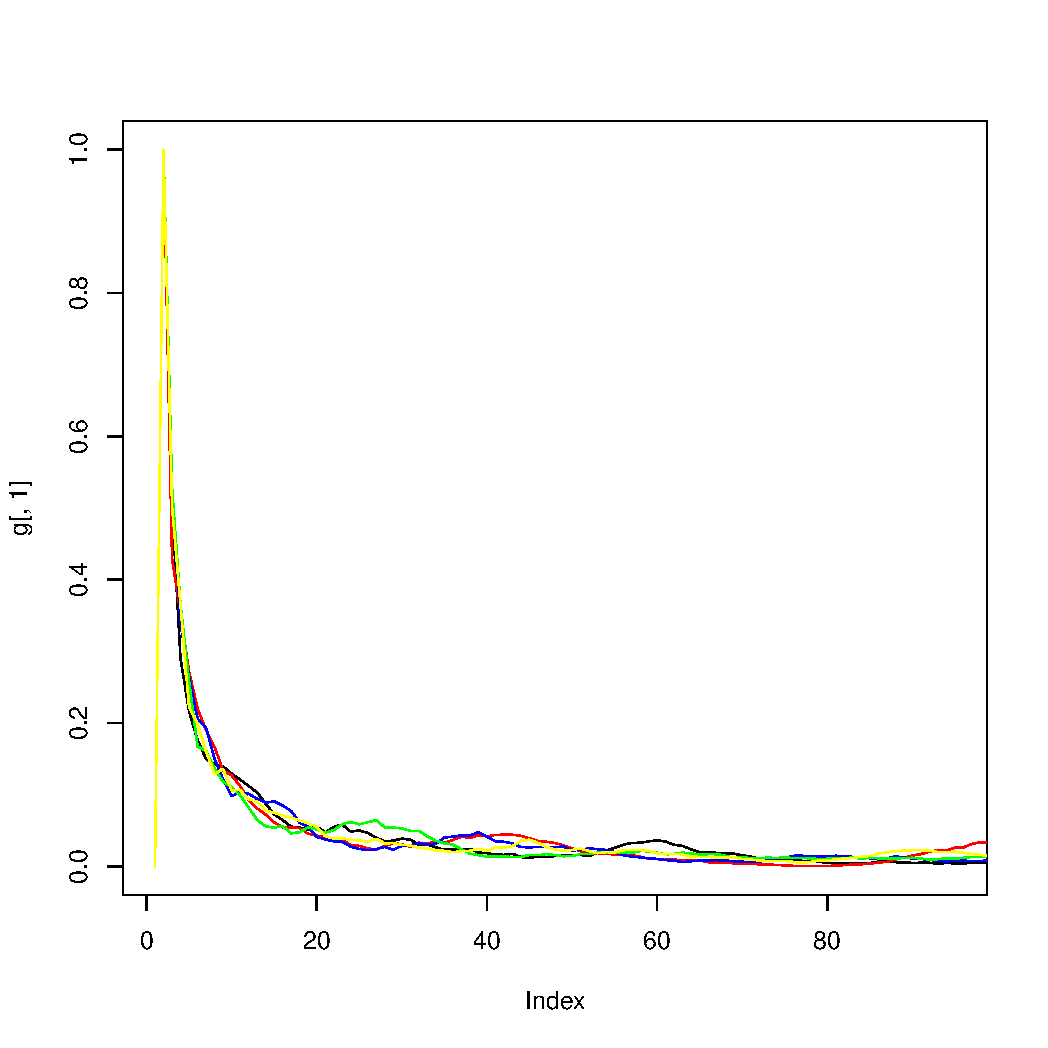
\includegraphics[width=3in]{growthres.pdf}
\end{center}
\caption{Growth Rates Per Area}
\end{figure}
\begin{figure}[H]
\begin{center}
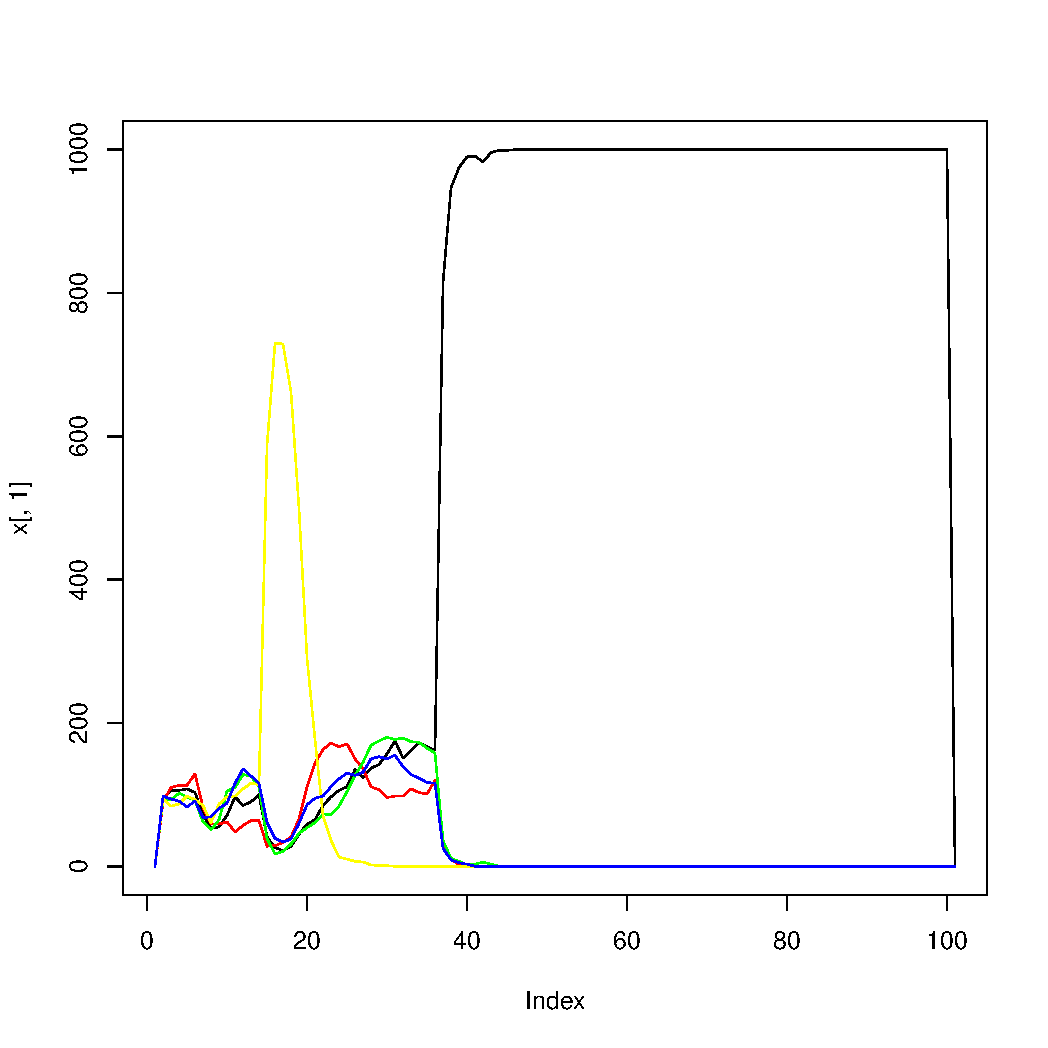
\includegraphics[width=3in]{newres_paradigm.pdf}
\end{center}
\caption{Paradigm Shift Model: New Research Per Area}
\end{figure}
\subsection{Analysis of the results}
\begin{enumerate}
\item
As expected in the base model we find that there are cycles in the number of papers written in a given area. These cycles are driven by the relative growth rates of the different areas which determine the probability of a researcher choosing the area s/he wants to works in. As discussed before researchers area attracted to high growth areas but once too many researchers enter a given area, the total number of papers in the field increases leading to lower growth rates in subsequent periods
\item
In the model with paradigm shift we find that the popularity of a given area (higher growth rate) leads to a greater chance of a game changer which leads to a growth rate of 100$\%$ in that period. Till a paradigm shift occurs the model shows the usual cycles, however once a paradigm shift does take place it increases the possibility of future paradigm shifts. This can lead to a situation where a given area attracts all the best brains, and finally all the brains in the discipline and the remaining research areas find no takers. 
\end{enumerate}

\section{Modeling research choice between disciplines}
For our second model, we focus on the benefits of doing interdisciplinary research. Here, instead of modeling agent choice between sub-disciplines, we allow agents either to do research within their own discipline or to collaborate with other agents in interdisciplinary research. We model three different strategies in an agent-based framework: \emph{Grinders}, who never choose to do interdisciplinary research; \emph{Interdisciplinarians}, who always choose to do interdisciplinary research; and \emph{Pragmatists}, who only choose to do interdisciplinary research when their own discipline is growing at a rate (as measured above) faster than the average rate of growth of academia.

\subsection{Model design}


This model is designed to test the relative success of the three research strategies across various leves of `ecosystem diversity,' or the number of possible research disciplines. More disciplines should represent more opportunities for strict Interdisciplinarians and academic Pragmatists to enter into interdisciplinary research, and thus circumvent the stagnation of their own disciplines.

Researchers produce one paper a year, and each discipline has a growth-rate which is the current number of researchers divided by the total number of previous papers since the start of the model. Eventually, this model may be used to explore the relationship between `institutional richness' (propensity for paradigm-shifting papers) and the success of different research strategies.

The simulation is initiated with various parameters, including the number of academics and the number of disciplines. Initial academics are assigned a strategy and discipline randomly according to a uniform distribution.

\begin{table}[H]
\begin{center}
\caption{Parameters of the simulation, and their values in the runs presented here.}
\label{tab:1}
\begin{tabular}{lrl}
  \hline
 Parameter & Value(s) & Description \\ 
  \hline
N & 1000 & Number of agents \\
M & 1:20 & Number of disciplines \\
Gi & 1/3 & Initial proportion of Grinders\\
Ii & 1/3 & Initial proportion of Interdisciplinarians\\
Pi & 1/3 & Initial proportion of Pragmatists\\
t & 100 & Number of academic generations\\
   \hline
\end{tabular}
\end{center}
\end{table}

The following occurs each time-step:
\begin{enumerate}
\item Growth-rates are calculated for each discipline.
\item Academic Pragmatists assess their own discipline’s growth-rate, and compare it to the mean rate of all disciplines; if a pragmatist's discipline is doing worse than the mean, they will attempt to do interdisciplinary research. All Interdisciplinarians also enter into the inter-disciplinary 'pool.'
\item Researchers in the new inter-disciplinary `pool' (some pragmatists and all interdisciplinarians) are randomly paired with one another, not allowing for pairs within the same discipline.
\item `Payoffs' go to each agent as a function of their discipline’s growth-rate, or as the mean growth rate of disciplines in an inter-disciplinary pair. Unpaired Interdisciplinarians or interdisciplinary Pragmatists recieve a payoff of zero.
\item Academic progeny (successful PhDs) are `birthed' to academics via a random draw with replacement from the previous generation, weighted by each academic's payoff.
\end{enumerate}

\subsection{Results}
As hypothesized, the success of strict Interdisciplinarians and academic Pragmatists improves as the number of disciplines increases. In a model with just two disciplines (Figure \ref{fig:1}), Interdisciplinarians initially compete with Grinders and Pragmatists, but as the balance of Interdisciplinarians between the two disciplines becomes less equal, Interdisciplinarians are increasingly selected against. Academic pragmatists are also all but eliminated from the discipline with the slower growth-rate, and pragmatists from the other discipline will never seek to do interdisciplinary research.

\begin{figure}[H]
\centering
\small
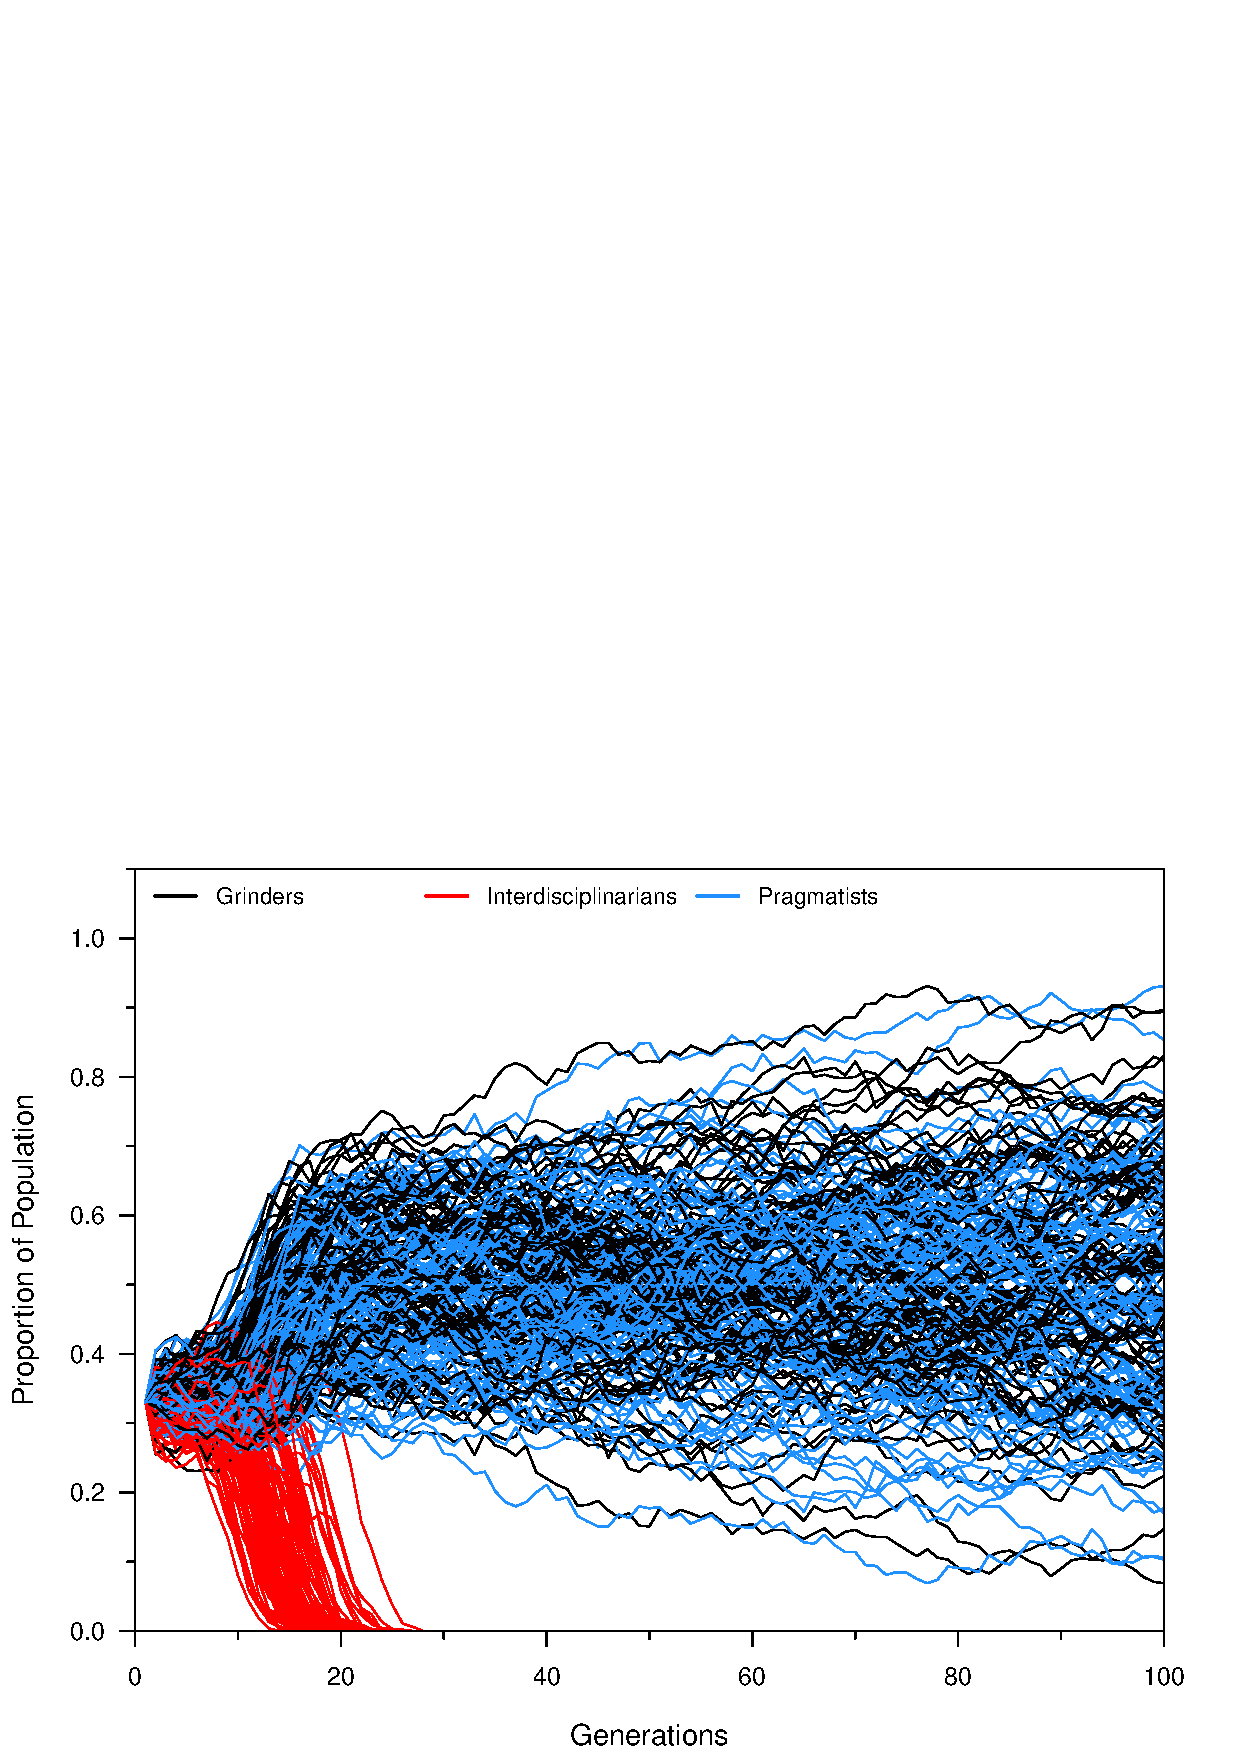
\includegraphics{Grinders-002}
\caption{Relative success of each strategy when M=2 (100 runs).}
\label{fig:1}
\end{figure}

In a model with just ten disciplines (Figure \ref{fig:2}), Interdisciplinarians are able to compete with Grinders and Pragmatists for a longer period than the two-discipline model, and are even sometimes able to dominate the population. As disciplines' populations wane to zero, however, the interdisciplinarians suffer the same as before. Interdisciplinarians are sometimes able to come to dominate the population, though, if they happen to take over the last discipline. Their payoffs drop to zero, but as they have no competition from other strategies, they remain in the population. The random absolute success by Interdisciplinarians is even more likely to occur as the number of disciplines grows (Figure \ref{fig:3}). Obviously, adding mutation to the simulation would abolish this trend, as a single Grinder or Pragmatist will be able to invade a population of Interdisciplinarians in a one-discipline system.

\begin{figure}[H]
\centering
\small
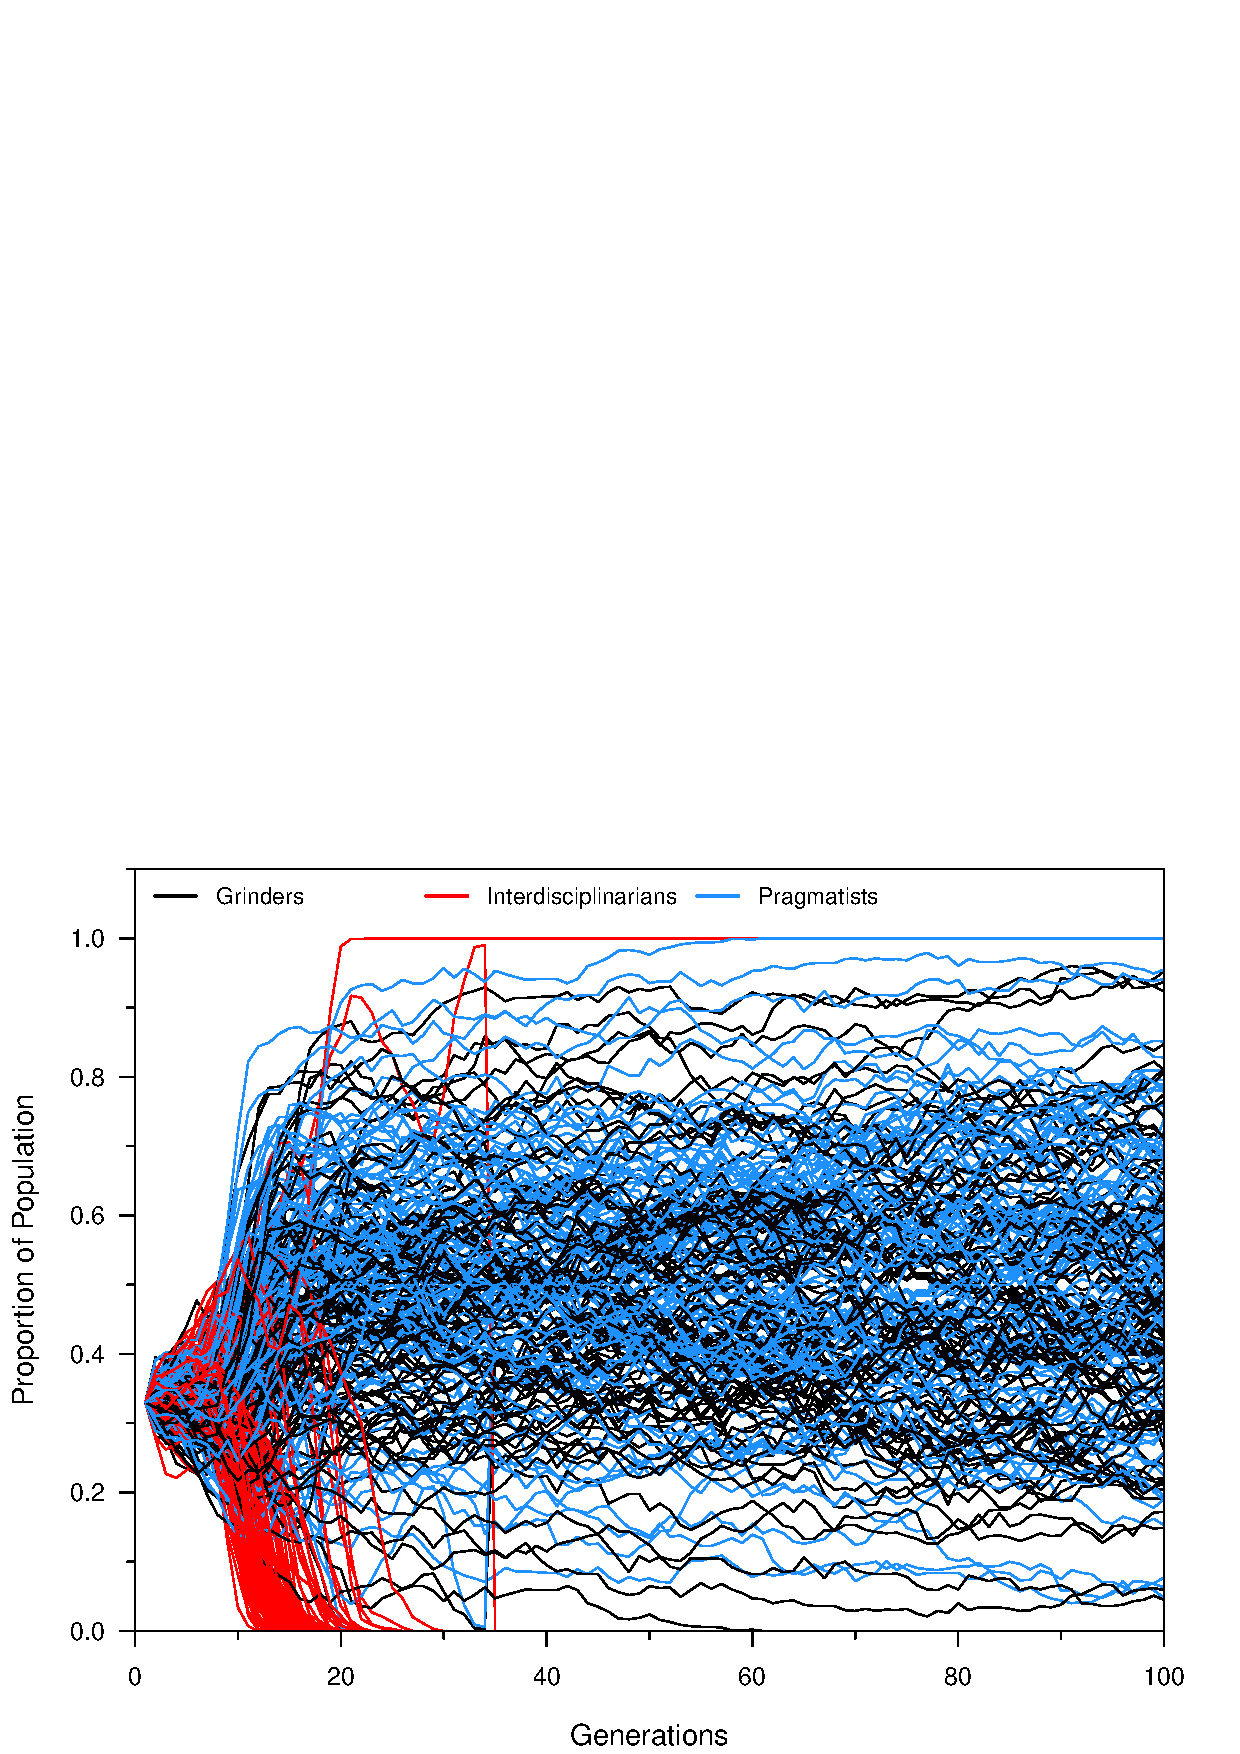
\includegraphics{Grinders-003}
\caption{Relative success of each strategy when M=10 (100 runs).}
\label{fig:2}
\end{figure}

\begin{figure}[H]
\centering
\small
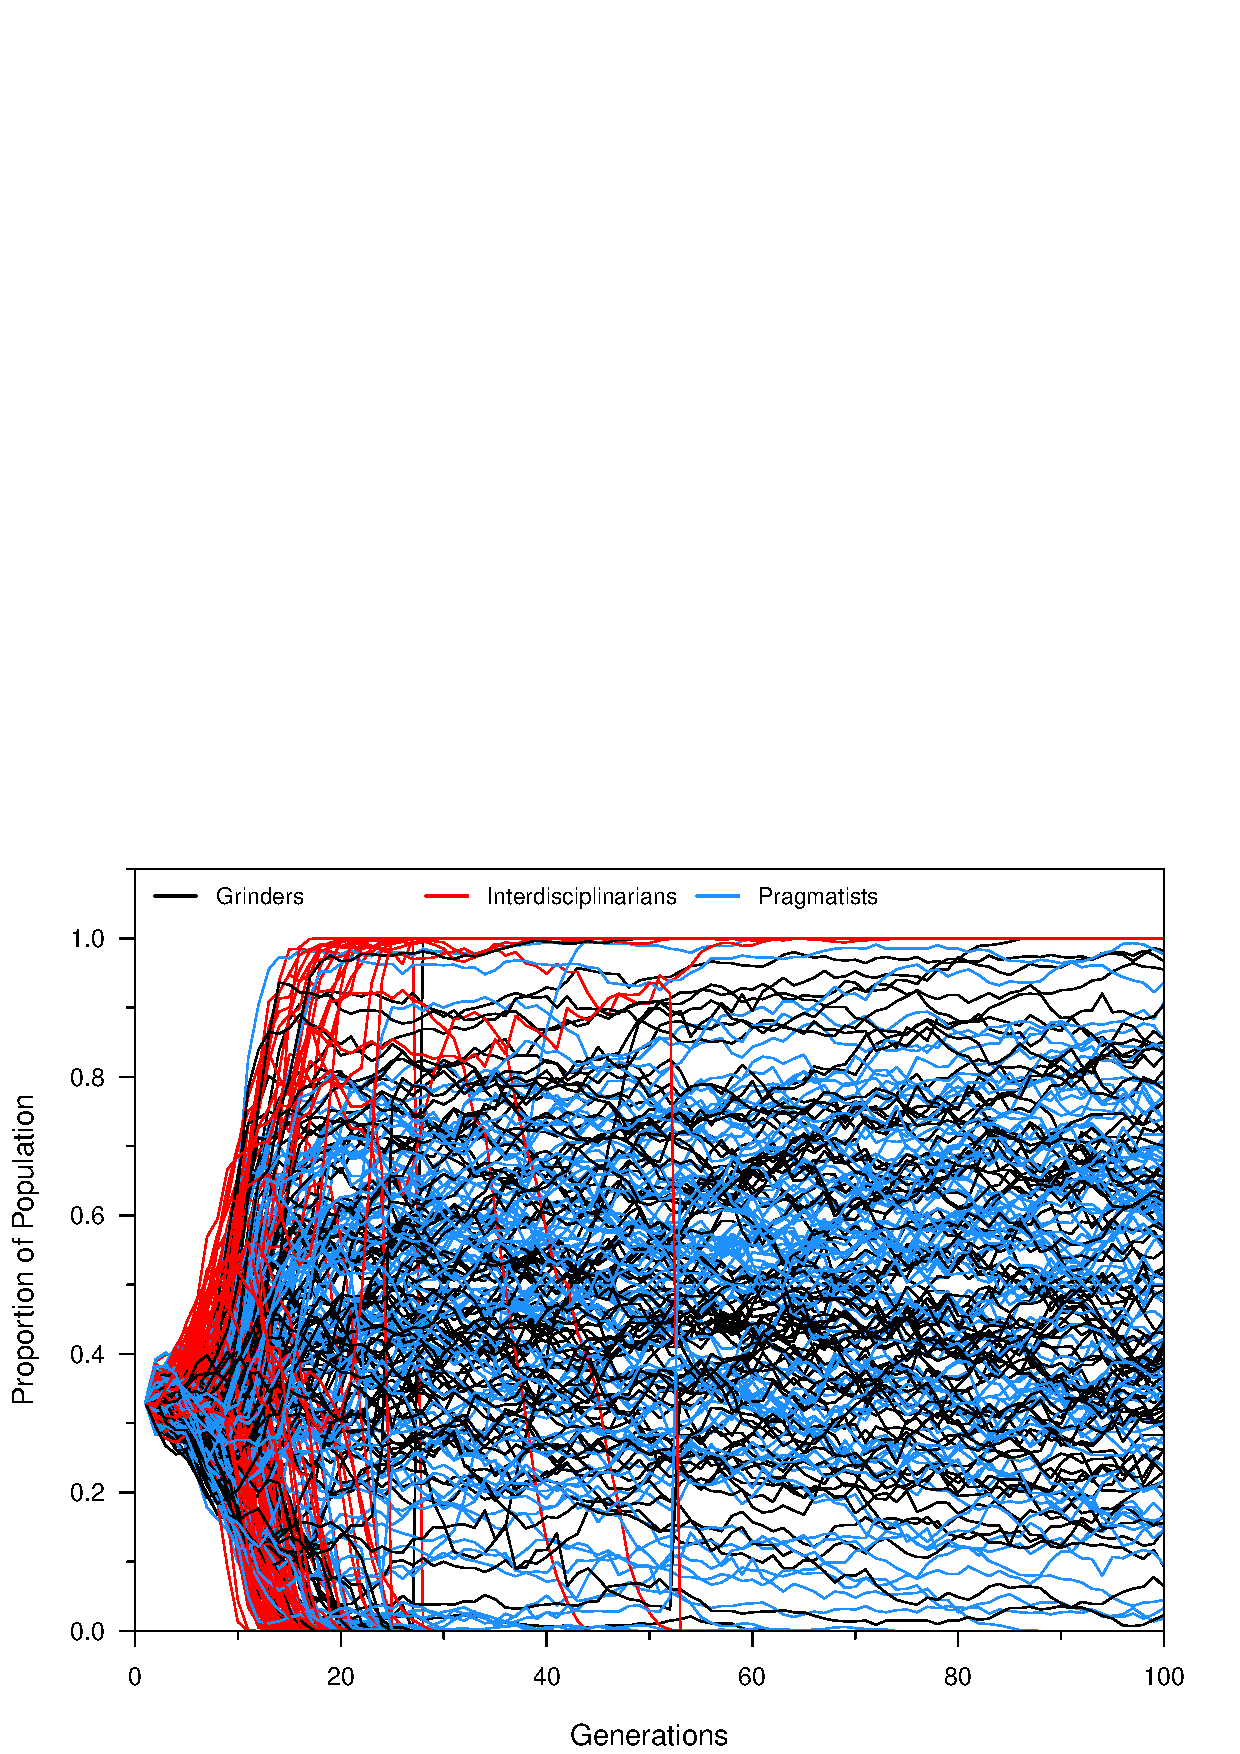
\includegraphics{Grinders-004}
\caption{Relative success of each strategy when M=20 (100 runs).}
\label{fig:3}
\end{figure}

Discipline survival is very low in this model (Figure \ref{fig:4}), which is a product of not including a `rejuvenating' process for disciplines, such as the paradigm shift noted above. Agents in disciplines that are initialized with more agents (randomly) are at a fitness disadvantage, thus leading to discipline elimination.

\begin{figure}[H]
\centering
\small
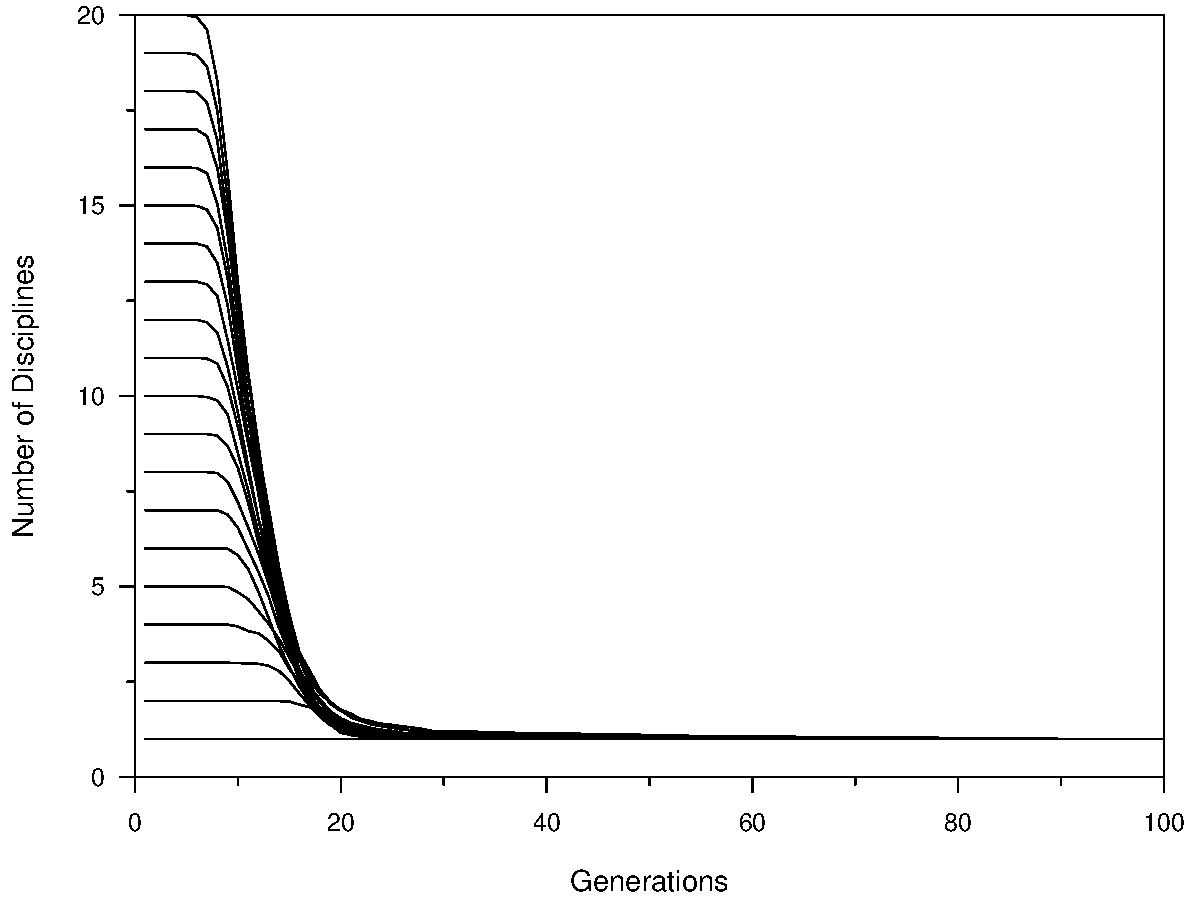
\includegraphics{Grinders-005}
\caption{Survival of disciplines after 100 timesteps. These curves represent the means of 100 runs at each M[1,20]}
\label{fig:4}
\end{figure}

\section{Possible Extensions and Other Applications}
Some directions that we can look at are:
\begin{enumerate}
\item
In the model with paradigm shift we can introduce the possibility of researchers randomly choosing a field that has died out, thus rejuvenating the field for future generations.
\item
We can also introduce a damping parameter that helps reduces the likelihood of serial paradigm shifts.
\item
Applications in Marketing: In markets with competing brands, especially technology-oriented products, companies compete for the best brains in the business (researchers and technicians who can come up with new innovations). We expect the balance to shift between different companies until the time that a particular brand comes up with a highly innovative product which becomes a game changer. The product/brand then becomes the market leader and also starts attracting all the best brains in the business, eventually becoming a giant. For example: Apple Products.
\item
Finally, our second model may be applicable to anti-trust policy in business, in that more corporations not only allow for more workers, but also support a greater diversity of worker types. With more competition, slackers (strict Interdisciplinarians) become employable.
\end{enumerate}

\end{document}

